\documentclass[rnaas]{aastex701}

\shorttitle{A Candidate Assessment of TOI-3492.01}
\shortauthors{\c{S}en}

\begin{document}

\title{A Six-Sector TESS Candidate Assessment of TOI-3492.01}

\author{Furkan \c{S}en}
\affiliation{Department of Astronomy and Space Sciences, Ankara University, Ankara, Turkey}
\email{furkan@fezadan.org}

\begin{abstract}
We assess the TESS Object of Interest TOI-3492.01 (TIC 81077799) using six
public 120-s SPOC light curves spanning five years. A transit-like signal at the
official 9.2224171-d ephemeris recurs in every sector. A circular fit to folded,
8-minute-binned photometry is retained only as a descriptive reference: its
formal intervals do not include the observed sensitivity to the fitting window,
baseline, and correlated residual noise. Archival SPOC diagnostics, Gaia DR3,
and first-pass TESS difference images provide useful screening information but
do not localize the source at calibrated confidence. We therefore report
TOI-3492.01 as an unvalidated, unconfirmed transit-like candidate. If the event
is planetary, occurs on TIC 81077799, and catalog single-star assumptions hold,
its diagnostic radius scale is compatible with a giant companion. Targeted
imaging, spectroscopy, and radial velocities are required before stronger
interpretation.
\end{abstract}

\keywords{Exoplanet detection methods (489) --- Transit photometry (1709) ---
Exoplanet candidates (1801) --- TESS (1685)}

\section{Observations and Candidate Assessment}

TOI-3492.01 is associated with TIC 81077799, a bright ($T=8.45$) evolved-host
candidate. We retrieved the public SPOC PDCSAP 120-s light curves from Sectors
37, 63, 64, 90, 99, and 100 through MAST using \texttt{lightkurve}
\citep{Jenkins2016,Lightkurve2018}. The corrected reference product contains
102\,502 finite measurements. Each sector was normalized independently near the
official ephemeris, and positive outliers were removed without applying a
transit-suppressing flattening operation.

A targeted BLS recovery finds a maximum at 9.222 d, the nearest grid point to
the official $P=9.2224171$ d period. The fixed-window robust depth is
$2694\pm26$ ppm, consistent in scale with the official 3109.8-ppm depth. All
six sectors contain a transit-like feature at the expected phase. Their formal
depths range from 2490 to 2874 ppm and reject a constant-depth model
($\chi^2=29.85$ for five degrees of freedom). This heterogeneity is not assigned
an astrophysical cause because aperture, background, reduction, and residual
noise effects remain viable alternatives.

Figure~\ref{fig:fold} shows the folded, 8-minute-binned data used for the
descriptive circular reference calculation. With fixed quadratic limb darkening,
that calculation gives
$R_p/R_\star=0.05472\pm0.00049$, $a/R_\star=10.60\pm0.45$, and
$b=0.705\pm0.032$. These are not adopted native-cadence measurements. A
separate fit with LDTk-derived Gaussian priors on the Kipping $q_1,q_2$
limb-darkening parameters yields $R_p/R_\star=0.05496$, $a/R_\star=10.38$, and
$b=0.720$; the free and fixed limb-darkening results agree within the
descriptive uncertainties. A
separate 13-h total-width fit shifts $R_p/R_\star$ by 1.95 reference-posterior
half-widths, and the attempted native-cadence noise analysis fails its
residual-correlation gate. The reference values consequently provide a useful
scale description, not a precision system solution.

The reference calculation fixes LDTk/PHOENIX quadratic limb darkening. The
target's metallicity is not measured, and limb-darkening, atmosphere-grid, and
stellar-model uncertainty are not propagated into a final transit posterior.
The short native-cadence chains do not meet the conservative $50\tau$
criterion; their intervals are omitted. A later sector-timescale Gaussian-process
method also failed its limited synthetic eligibility test, so no correlated-noise
model is adopted for the real data.

\begin{figure}[t]
\centering
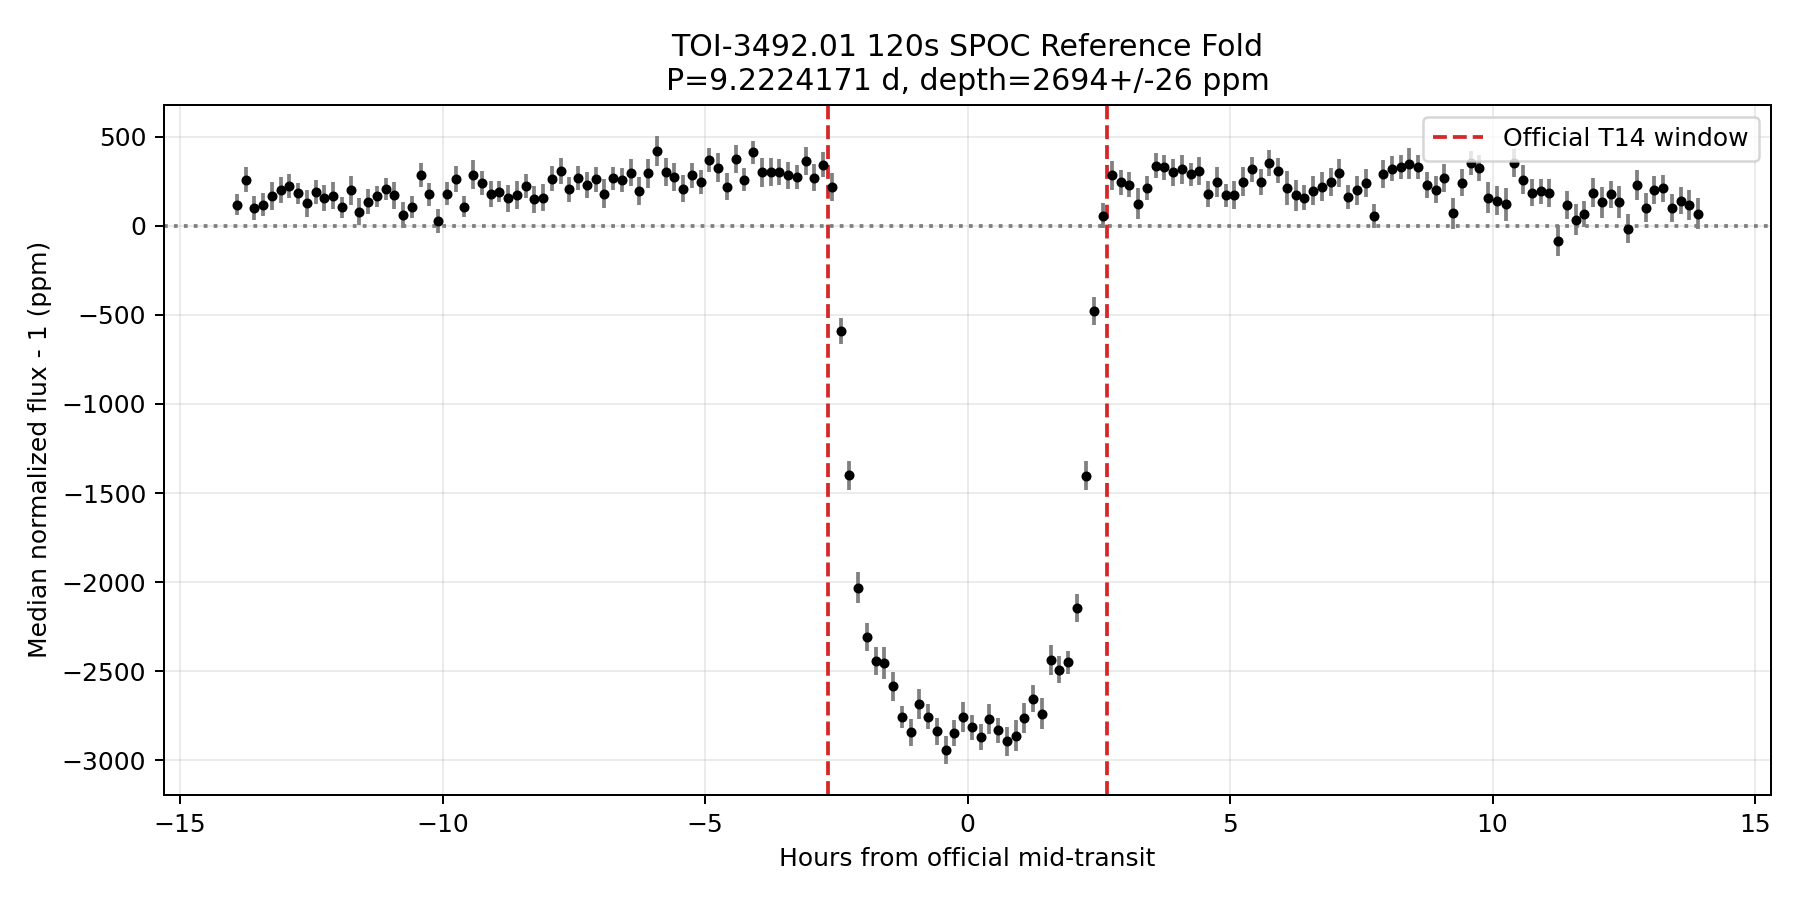
\includegraphics[width=\linewidth]{figures/toi3492_120s_reference_fold.png}
\caption{Six-sector corrected 120-s SPOC light curve folded on the official
ephemeris. Black points are binned photometry; red dashed lines mark the
official duration window. This visualization and its associated circular
reference calculation are not an adopted native-cadence posterior.}
\label{fig:fold}
\end{figure}

The TIC v8 catalog gives $R_\star=2.5926\pm0.1094\,R_\odot$,
$M_\star=1.25\pm0.19\,M_\odot$, and $T_{\rm eff}=6332\pm134$ K
\citep{Stassun2019}. If the event is planetary, originates on this catalog
target, and the single-star catalog model is appropriate, the reference radius
ratio implies $R_p=15.47\pm0.66\,R_\oplus$. This is a host-conditional scale,
not an unconditional companion-radius measurement.

We performed screening checks without converting them into a false-positive
probability. Odd and even fixed-window depths differ by $19$ ppm ($0.39\sigma$),
and a fixed phase-0.5 search gives $8\pm15$ ppm. Neither test has an
injection-calibrated sensitivity limit under the final noise model. Gaia DR3
shows no source within 42 arcsec bright enough to mimic the full signal as a
fully eclipsed contaminant; the nearest Gaia neighbor is 7.37 arcsec away and
10.65 mag fainter \citep{Vallenari2023}. First-pass difference-image centroids
fall within about one TESS pixel of the target, while public SPOC DV centroid
metrics are consistent with zero offset. These are encouraging diagnostics, but
they are not calibrated PRF localization and do not establish the sky source.
A Gaia source at 56.29 arcsec has a $G$-band flux ratio of 0.00431 and could in
principle mimic the observed dimming if deeply eclipsed. It is outside the
discrete SPOC aperture in all six sectors, but unmodeled PRF wings prevent that
geometry from excluding it. A per-pixel in-transit fractional-depth map yields a
flux-weighted centroid closer to the catalog target than to this neighbor in
four of six sectors, consistent at the individual-pixel level with a
target-region origin; this deepens but does not replace calibrated PRF
localization. We therefore report neither a TRICERATOPS-derived nor any other
formal false-positive probability: calibrated PRF localization and a
high-resolution contrast curve are unavailable.

TOI-3492.01 is thus a persistent transit-like candidate, not a statistically
validated or dynamically confirmed planet. The most useful next observations are
time-series imaging during transit for source attribution, high-resolution
imaging for unresolved companions, reconnaissance spectroscopy for the host, and
epoch radial velocities for companion-mass constraints. The public TESS data
support this candidate assessment; they do not support a formal false-positive
probability, an eccentricity measurement, or a mass measurement.

\begin{acknowledgments}
This work used data from the TESS mission, funded by NASA's Science Mission
Directorate and available through MAST. This work also used \texttt{lightkurve}
and Gaia DR3 data processed by the Gaia Data Processing and Analysis Consortium.
\end{acknowledgments}

\facilities{TESS, Gaia}
\software{Lightkurve \citep{Lightkurve2018}, batman \citep{Kreidberg2015}}

\bibliographystyle{aasjournalv7}
\bibliography{references}

\end{document}
